\chapter{Servrová časť}
Hlavnou funkcionalitou tejto časti je obslúžiť požiadavky prichádzajúce ako http volania, spracovať ich a vrátiť výsledok vo formáte JSON. Backend sa teda priamo nestará o obslúženie užívateľských akcií, ani o routovanie a len odpovedá na volania z klienta. V REST api vystavujeme tieto metódy:

\newcolumntype{M}[1]{>{\arraybackslash}m{#1}}
\newcolumntype{N}[1]{>{\centering\arraybackslash}m{#1}}
\begin{table}[htbp]
 	\centering
\begin{tabular}{| M{1.5cm} | M{5cm} | N{4.5cm} |}
\hline
Metóda & \multicolumn{1}{c|}{Url}   & \multicolumn{1}{c|}{Akcia}                \\ \hline
POST   & /api/task/                 & Spustí analýzu                            \\ \hline
GET    & /api/task/\{pk\}/status/   & Vráti stav analýzy                        \\ \hline
GET    & /api/patterns/             & Vráti parsovacie vzory                    \\ \hline
POST   & /api/patterns/             & Finalizuje parsovací vzor                 \\ \hline
DELETE & /api/patterns/\{pk\}/      & Zmaže vzor                                \\ \hline
GET    & /api/patterns/\{pk\}/lines & Vráti správy parsovacieho vzoru           \\ \hline
GET    & /api/export-patterns/      & Transformuje a exportuje parsovacie vzory \\ \hline
GET    & /api/sources/              & Vráti zdroje zdroje správ                 \\ \hline
GET    & /api/autocomplete/source   & Doplní názov zdroja správ                 \\ \hline
GET    & /api/autocomplete/version  & Doplní verziu zdroja správ                \\ \hline
GET    & /api/regex-groups/         & Vráti sady regulárnych výrazov            \\ \hline
POST   & /api/regex-groups/         & Importuje sadu regulárnych výrazov        \\ \hline
DELETE & /api/regex-groups/\{pk\}/  & Zmaže sadu regulárnych výrazov            \\ \hline
\end{tabular}
% \end{minipage}
 \caption{Frekvenčná tabuľka pre algoritmus Nagappan-Vouk}
\label{fig:nagappan}
\end{table}
%\end{figure}
 
 
Pri implementácií sme sa intenzívne spoliehali framework Django. Django obsahuje veľké množstvo modulov, z ktorých sme v našej práci síce využili len malú podmnožinu, ale zásadne nám zjednodušila celú implementáciu. Funkcionalita je rozdelená do samostatných súborov alebo modulov pre jednoduchý a prehľadný kód.

\subsection{Django ORM}
Pre prístup k dátam z databázy je v celej aplikácii použité objektovo relačné mapovanie zakomponované priamo v Djangu. Využitie Django ORM vo väčšine prípadov vývojára úplne odprostí od potreby implementovať vrstvu pre prístup k dátam, ako je zvyklé napr. v Jave alebo \#C. Django ORM používa potomkov triedy \emph{django.db.models.Model}, ďalej nazývaných ako modely, na zadefinovanie štruktúry dát a pôsobí ako jediný prístupový bod k dátam. Každý model reprezentuje tabuľku v databáze a jeho objekt tohto typu jeden riadok v databáze. 

\begin{figure}[htbp]
\centering
\begin{minipage}{0.9\textwidth}
\lstset{columns=flexible,breaklines=true,breakatwhitespace=true, showstringspaces=false}
\begin{lstlisting}
class Source(models.Model):
    source = models.CharField(max_length=255, blank=False, db_index=True)
    version = models.CharField(max_length=50)

    class Meta:
        unique_together = ('source', 'version')
\end{lstlisting} 		
\end{minipage} 
\caption{Django ORM model typu Source}
\label{fig:static-analysis}
\end{figure}

\subsection{Django migrations}
Na vytvorenie databázového schématu používame Django migrations. Použitím Django migrations vývojári nemusia písať ddl scripty a modelujú schéma vytváraním tried v jazyku python. Prvotné schéma je vygenerované automaticky, každá ďalšia zmena kódu spôsobí vygenerovanie novej migrácie, ktorá je následne aplikovaná na databázové tabuľky. Tento spôsob sa ukázal ako veľmi nápomocný v deployment scriptoch, kde jednoducho spustíme migráciu príkazom \emph{python manage.py migrate} a nepotrebujeme dodatočného sql klienta na vytvorenie schématu. Zároveň týmto spôsobom vieme do aplikácie aj vložiť iniciálne data.

\begin{figure}[htbp]
 \centering 
 \begin{minipage}{0.95\linewidth}
 	\centering
 	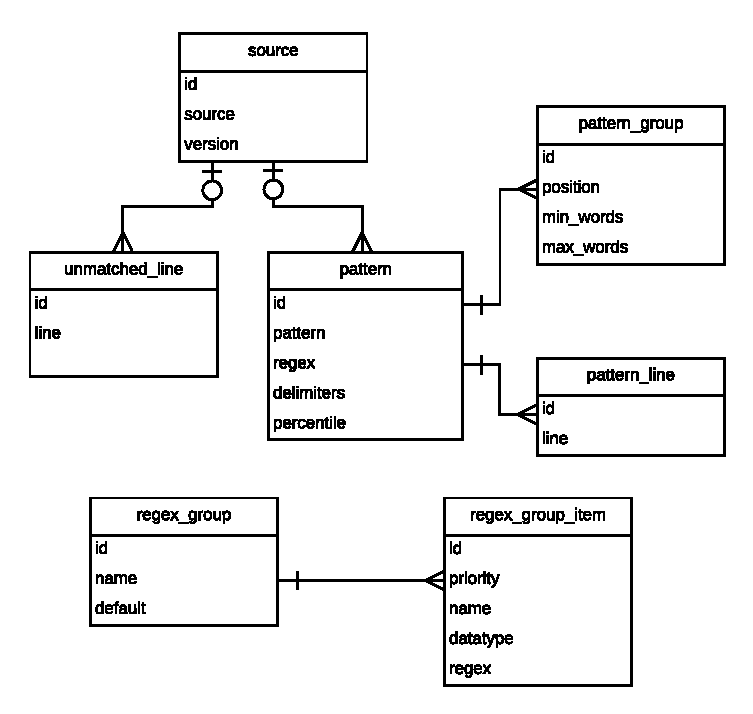
\includegraphics[width=\textwidth]{Images/thesis-erd.pdf}	
 \end{minipage}
  \caption{ERD diagram}
  \label{fig:use-cases}
\end{figure}

\subsection{Implementácia Extended Nagappan-Vouk}
Implementácia sa snaží byť čo najrýchlejšia, preto používame knižnicu \emph{multiprocessing}. Väčšina vykonávaných metód najprv rozdelí problém na menšie časti, spočíta výsledok podproblému v novom procese a následne problém spojí. 
\par  Začína predspracovaní, v ktorom pre každú správu hľadáme sekvenčným prechodom cez už uložené parsovacie vzory ten správny. Ak existuje daná správa je z ďalšieho spracovania vylúčená. Uznávame, že táto operácia nie je veľmi efektívna ako už bolo zmienené v \ref{sec:data-mining} a s narastajúcim počtom uložených správ značne zhorší celkový čas spracovania, preto implementácia tejto operácie môže byť v budúcnosti  jednoducho zameniteľná za riešenie založené na REtrie. Nasleduje samotný beh algoritmu, ktorého výsledky sú uložené do Redisu. Ako návratova hodnota je použitý objekt ktorý obsahuje štatistiku vytvorenú z týchto výsledkov a textovú reprezentáciu parsovacích vzorov.

\subsection{Prevod medzi formátmi parsovacích vzorov}
\label{sec:format-transformation}

Pri prevode medzi týmito formátmi potrebujeme mať vopred známu sadu typov regulárnych výrazov, voči ktorým budeme konverziu prevádzať. Je žiadúce aby táto sada nebola konštantná pre všetky parsovacie vzory, ale aby bolo možné ju zadať pre vybrané parsovacie vzory. Z tohto dôvodu nie je transformácia medzi formátmi prevádzaná pri uložení parsovacie vzoru, ale je vykonaná on demand pre zadanú sadu typov algoritmom \ref{fig:pattern-transformation}

\begin{figure}[htbp]
\centering
\begin{minipage}{0.9\textwidth}
\lstset{columns=flexible,breaklines=true,breakatwhitespace=true, showstringspaces=false}
\begin{lstlisting}
def transform(pattern, pattern_lines, regex_types):
    types_tab = build_types(pattern, pattern_lines, regex_types)
    transformed_patterns = {}, pattern_idx = 0
    for line_key, types in types_tab.items():
        idx = 0
        replacements = []
        replacement = ''
        for words_in_groups in line_key.split():
            replacement = ''
            for words_in_group in words_in_groups:
                replacement.append('%{{{name}:var{idx}}}'
                    .format(name=types[idx], idx=idx))
                idx += idx
            replacements.append(replacement)   
        transformed_patterns['pattern' + pattern_idx] = replace_groups_text(pattern, replacements)
    return transformed_patterns

def build_types(pattern, pattern_lines, regex_types):
    pattern_types = {}
    for line in pattern_lines:
        pattern_match = pattern.match(line)
        types = [], keys = []
        pattern_groups = pattern_match.groups()
        for pattern_group in pattern_groups:
            words = pattern_group.split()
            for word in words:
                types.append(
                   find_first_suitable_regex_type(word, regex_types))
            keys.append(str(len(words)))
        line_key = ','.join(keys)
        update_types(pattern_types, line_key, types)
    return pattern_types
\end{lstlisting} 		
\end{minipage} 
\caption{Algoritmus transformácie parsovacieho vzoru na REtrie formát}
\label{fig:pattern-transformation}
\end{figure}

Hlavný rozdiel medzi popisovanými formátmi je ten, že pokým nativný formát algoritmu Extended Naggap-Vouk skracuje výskyt viacerých parametrov v rade, REtrie formát tento zápis nepozná. Preto vo výsledku z jedného parsovacieho vzoru, môže vzniknúť až 
\begin{align*}
\prod_{group \in groups} group.upper\_bound - group.lower\_bound
\end{align*}
nových vzorov. Ďalší rozdiel je neprítomnosť typu parametra v pôvodnom formáte.
